\subsection{Task 5: Triển khai TinyML và đánh giá độ chính xác}
\subsubsection{Tổng quan luồng thực thi của TinyML:}
Toàn bộ hệ thống được thiết kế theo một luồng khép kín từ môi trường vật lý đến mô hình toán học và quay trở lại thiết bị nhúng. Kiến trúc này được chia thành ba giai đoạn (Phase) chiến lược, đảm bảo tính minh bạch và tối ưu hóa tài nguyên cho vi điều khiển ESP32.

\subsubsection*{Phase 1: Luồng dữ liệu (Data Pipeline)}
Giai đoạn này đóng vai trò là "cầu nối" chuyển đổi các tín hiệu vật lý thành tri thức số học.
\begin{itemize}
    \item \textbf{Số hóa tín hiệu:} Dữ liệu điện tử từ cảm biến được thu thập qua cổng Serial dưới dạng log thô thông qua \texttt{collect\_from\_log.py}.
    \item \textbf{Cấu trúc hóa và Gán nhãn:} Trọng tâm của giai đoạn này là biến các dòng văn bản rời rạc thành tập dữ liệu cấu trúc (\texttt{.csv}). Sử dụng \texttt{extract\_ready\_data.py}, hệ thống áp dụng các quy tắc logic nghiệp vụ (Heuristics) để tự động gán nhãn cho từng cặp giá trị (Nhiệt độ, Độ ẩm), tạo ra "Ground Truth" cho quá trình huấn luyện AI.
\end{itemize}

\subsubsection*{Phase 2: Luồng Học máy (ML Pipeline)}
Được ví như "bộ não" của hệ thống, nơi diễn ra quá trình chọn lọc tự nhiên giữa các thuật toán học máy.
\begin{itemize}
    \item \textbf{Bộ lọc ESP32 Score:} Thay vì chỉ tối ưu hóa độ chính xác, hệ thống sử dụng một bộ chỉ số đánh giá khắt khe trong \texttt{evaluate\_models\_comprehensive.py}. Mô hình được chọn phải thỏa mãn sự cân bằng giữa độ chính xác, tốc độ suy luận và kích thước bộ nhớ.
    \item \textbf{White-box Export:} Điểm khác biệt cốt lõi là việc không sử dụng các tệp mô hình \texttt{.tflite} nặng nề. Thay vào đó, \texttt{export\_naive\_bayes.py} trích xuất các tham số xác suất (Theta, Variance) và dịch chúng trực tiếp thành ngôn ngữ C (\texttt{.h}), cho phép thực thi suy luận bằng các phép toán cơ bản.
\end{itemize}

\subsubsection*{Phase 3: Triển khai và Xác thực (Deployment \& Validation)}
Giai đoạn cuối cùng thực hiện việc thực thi mô hình đồng thời trên hai môi trường để đảm bảo tính nhất quán.
\begin{itemize}
    \item \textbf{Nhánh Kiểm thử (PC):} \texttt{test\_naive\_bayes.py} sử dụng các tham số đã xuất để giả lập suy luận trên máy tính, giúp kiểm tra tính đúng đắn của thuật toán trước khi nạp vào phần cứng.
    \item \textbf{Nhánh Thực thi (ESP32):} Mô hình được tích hợp vào tác vụ \texttt{tiny\_ml\_task} trong \texttt{tinyml.cpp}. Tại đây, vi điều khiển sử dụng chung "hệ quy chiếu toán học" với máy tính để đưa ra quyết định tại chỗ (At-the-edge) dựa trên dữ liệu cảm biến thời gian thực.
\end{itemize}

Sự phối hợp giữa ba giai đoạn này tạo nên một hệ thống TinyML tinh gọn, có khả năng vận hành bền bỉ trên các thiết bị IoT hạn chế về tài nguyên.
\begin{figure}[htbp]
    \centering
    % Cài đặt chiều rộng ảnh bằng 80% chiều rộng văn bản
    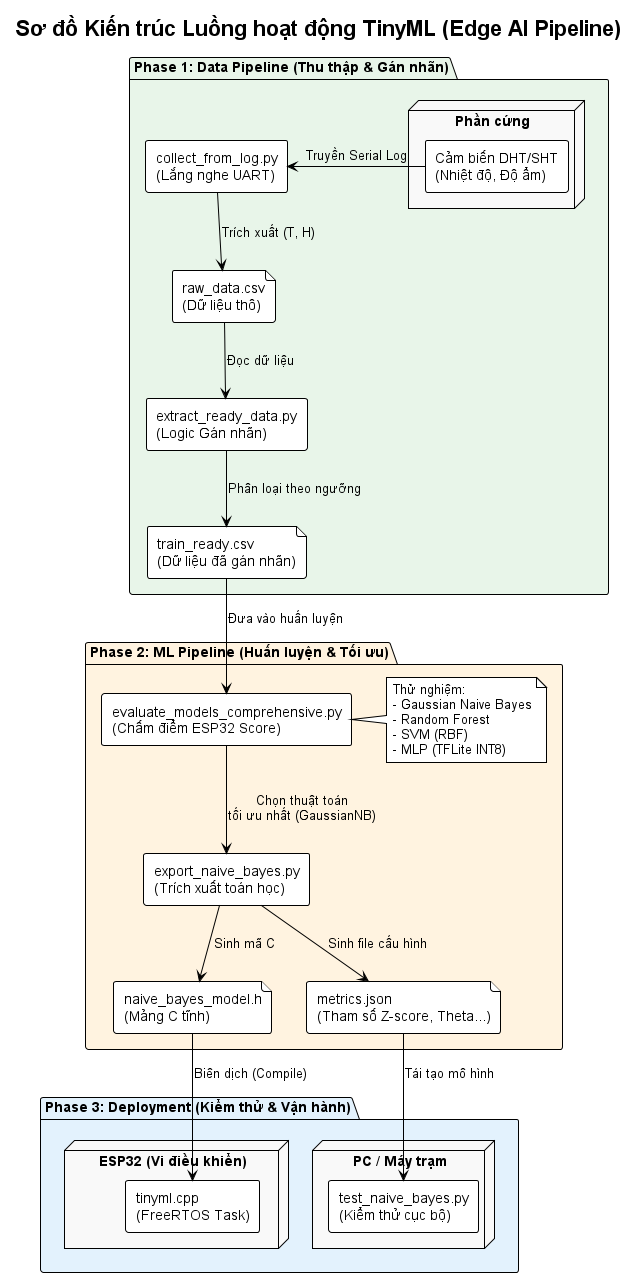
\includegraphics[width=0.7\textwidth]{picture/iot.png} 
    \caption{Tổng quan luồng thực thi của TinyML từ thu thập dữ liệu đến triển khai trên ESP32. }
    \label{fig:mips_datapath}
\end{figure}


\subsubsection{Thu thập dữ liệu từ cảm biến (Data Collection)}

Giai đoạn đầu tiên của hệ thống là thu thập dữ liệu thô từ cảm biến nhiệt độ và độ ẩm thông qua giao tiếp Serial. \texttt{collect\_from\_log.py} đóng vai trò là trình lắng nghe và xử lý dữ liệu từ vi điều khiển ESP32.

\begin{itemize}
    \item \textbf{Giao tiếp Serial:} Sử dụng thư viện \texttt{pyserial} để thiết lập kết nối UART với Baudrate mặc định là 115200. Hệ thống liên tục đọc các dòng log từ cổng chỉ định (ví dụ: COM4).
    \item \textbf{Cơ chế phân tích (Parsing):} Để đảm bảo tính linh hoạt, hệ thống hỗ trợ ba định dạng đầu vào khác nhau thông qua hàm \texttt{parse\_temp\_humi\_from\_line}:
    \begin{enumerate}
        \item \textbf{JSON:} Phân tích chuỗi có dạng \texttt{\{"temperature": X, "humidity": Y\}}.
        \item \textbf{Regex:} Sử dụng biểu thức chính quy \texttt{T\textbackslash s*=\textbackslash s*(...)\textbackslash D+H\textbackslash s*=\textbackslash s*(...)} để tìm các mẫu như "T=30.5 H=65.2".
        \item \textbf{CSV Fallback:} Nếu không khớp các định dạng trên, hệ thống sẽ tự động tách chuỗi bằng dấu phẩy và lấy hai giá trị cuối cùng.
    \end{enumerate}
    \item \textbf{Lưu trữ dữ liệu:} Dữ liệu sau khi trích xuất thành công được gắn nhãn thời gian thực (ISO 8601) và ghi nối tiếp vào tệp \texttt{raw\_data.csv} bằng \texttt{csv.DictWriter}.
\end{itemize}

Việc sử dụng \texttt{f.flush()} sau mỗi dòng ghi giúp đảm bảo dữ liệu không bị mất mát trong trường hợp kết nối Serial bị ngắt đột ngột.
\newpage
\subsubsection{Tiền xử lý và Gán nhãn dữ liệu (Data Preprocessing and Labeling)}

Sau khi thu thập được dữ liệu thô, bước tiếp theo là làm sạch và gán nhãn tự động để tạo ra tập dữ liệu sẵn sàng cho việc huấn luyện mô hình (train-ready). Quá trình này được thực hiện thông qua  \texttt{extract\_ready\_data.py}.

\begin{itemize}
    \item \textbf{Mục tiêu:} Chuyển đổi tệp \texttt{raw\_data.csv} thành \texttt{train\_ready.csv} bằng cách áp dụng các quy tắc logic nghiệp vụ để xác định trạng thái của hệ thống dựa trên thông số môi trường.
    \item \textbf{Quy tắc gán nhãn (Heuristic Labeling):} Hệ thống sử dụng hàm \texttt{classify\_label} để phân loại dữ liệu vào các nhãn mục tiêu:
    \begin{itemize}
        \item \textbf{Bật máy sưởi:} Khi nhiệt độ thấp hơn 24.0°C.
        \item \textbf{Bật điều hòa:} Khi nhiệt độ lớn hơn 33.0°C và độ ẩm nằm trong khoảng 50\% - 80\%.
        \item \textbf{Bật máy hút ẩm:} Khi nhiệt độ lớn hơn 33.0°C và độ ẩm vượt quá 80\%.
        \item \textbf{Không hợp lệ:} Dữ liệu nằm ngoài dải vật lý (0 - 100) hoặc thiếu giá trị.
        \item \textbf{Chế độ bình thường:} Các trường hợp còn lại trong dải đo cho phép.
    \end{itemize}
    
\end{itemize}



Kết quả của giai đoạn này là một tệp CSV gồm ba cột chính: \texttt{temperature}, \texttt{humidity}, và \texttt{label}, phục vụ trực tiếp cho các thuật toán học máy ở bước sau.

\subsubsection{Đánh giá và So sánh Mô hình (Model Benchmarking)}

Để tìm ra kiến trúc học máy phù hợp nhất cho phần cứng hạn chế tài nguyên, hệ thống tiến hành đánh giá toàn diện nhiều thuật toán khác nhau thông qua \texttt{evaluate\_models\_comprehensive.py}. Quá trình này không chỉ xét đến độ chính xác mà còn đặc biệt chú trọng vào tài nguyên hệ thống.

\begin{itemize}
    \item \textbf{Các mô hình thử nghiệm:} Hệ thống tiến hành huấn luyện và đối chiếu bốn mô hình đại diện:
    \begin{enumerate}
        \item Gaussian Naive Bayes (GaussianNB).
        \item Random Forest.
        \item Support Vector Machine (SVM) với nhân RBF.
        \item Multi-Layer Perceptron (MLP) - Kích thước được ước lượng bằng cách lượng tử hóa trọng số về INT8 theo chuẩn TensorFlow Lite.
    \end{enumerate}
    \item \textbf{Chỉ số đánh giá ML tiêu chuẩn:} Các mô hình được đo lường hiệu suất thông qua Độ chính xác (Accuracy), Precision, Recall, F1-Score (trung bình có trọng số) và diện tích dưới đường cong ROC (ROC-AUC). Hệ thống cũng sử dụng K-Fold Cross-validation (với $K=5$) để đánh giá tính ổn định của mô hình.
    \item \textbf{Chỉ số phần cứng (ESP32 Score):} Điểm đột phá của luồng công việc này là việc định nghĩa một công thức tính điểm (thang 100) dành riêng cho TinyML, bao gồm ba trọng số chính:
    \begin{itemize}
        \item \textbf{Độ chính xác (40\%):} Ưu tiên khả năng nhận diện đúng trạng thái.
        \item \textbf{Kích thước mô hình (30\%):} Dung lượng tính bằng KB. Mô hình $<100$KB được coi là lý tưởng; mô hình $>1000$KB bị trừ điểm mạnh do giới hạn bộ nhớ Flash/RAM của vi điều khiển.
        \item \textbf{Tốc độ suy luận (30\%):} Đánh giá thời gian dự đoán (ms) để đảm bảo đáp ứng thời gian thực.
    \end{itemize}
\end{itemize}

Kết thúc quá trình đánh giá, hệ thống kết xuất một bảng xếp hạng (Ranking) và báo cáo JSON chi tiết. Các biểu đồ so sánh trực quan (như \textit{Model Size Comparison} và \textit{ESP32 Score}) sẽ tự động được tạo ra nhằm hỗ trợ lập trình viên ra quyết định lựa chọn thuật toán triển khai cuối cùng.
\begin{figure}[htbp]
    \centering
    % Cài đặt chiều rộng ảnh bằng 80% chiều rộng văn bản
    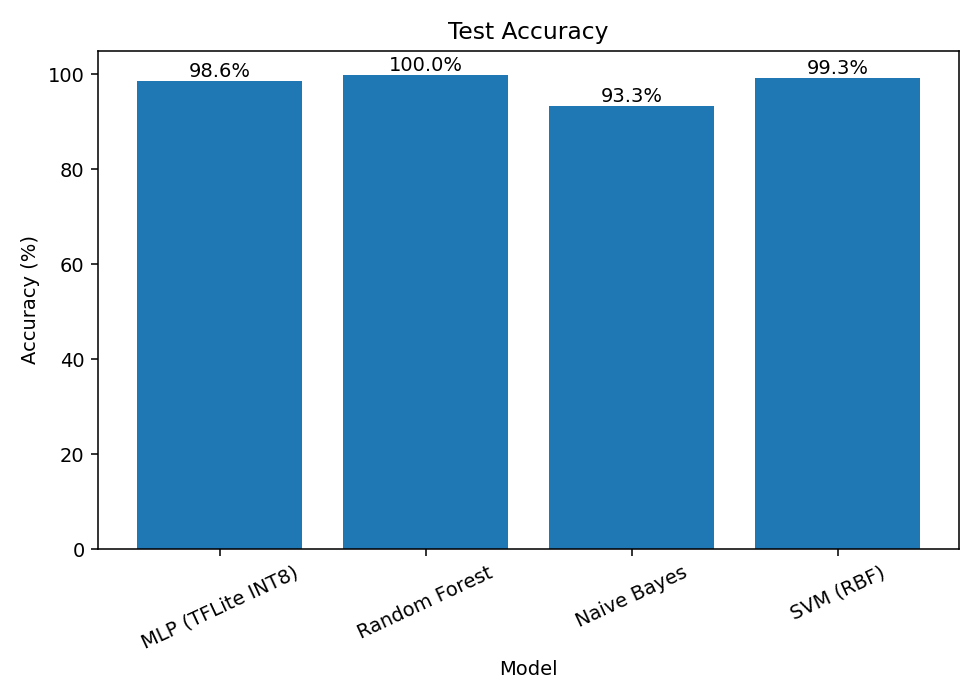
\includegraphics[width=0.8\textwidth]{picture/benchmark_accuracy.png} 
    \caption{Biểu đồ so sánh độ chính xác của các mô hình ML khác nhau trên tập dữ liệu huấn luyện. }
    \label{fig:mips_datapath}
\end{figure}

\begin{figure}[htbp]
    \centering
    % Cài đặt chiều rộng ảnh bằng 80% chiều rộng văn bản
    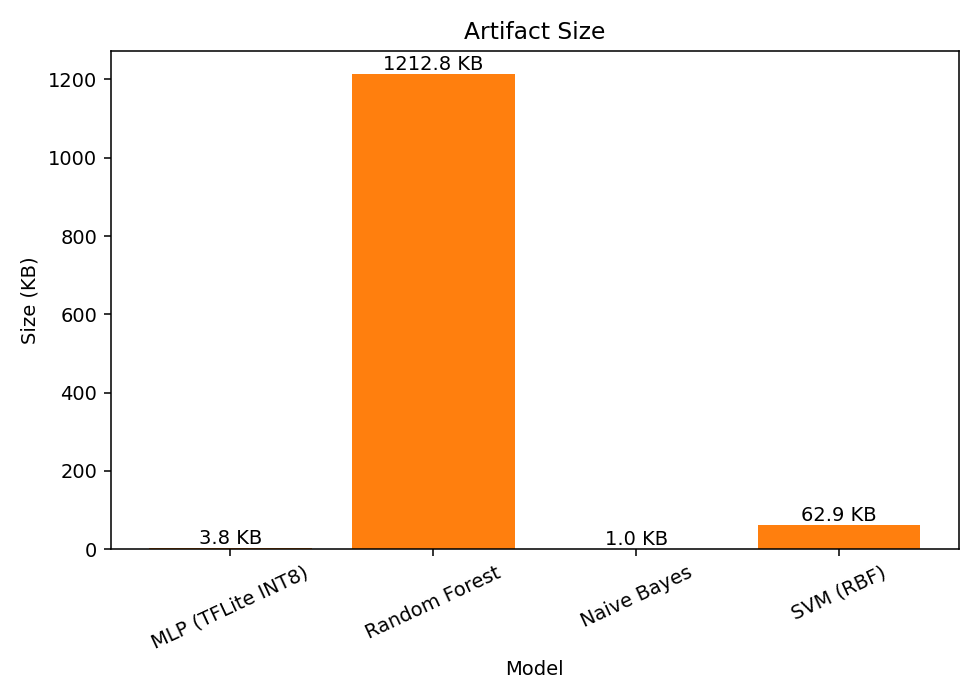
\includegraphics[width=0.8\textwidth]{picture/benchmark_artifact_size.png} 
    \caption{Biểu đồ so sánh kích thước mô hình của các mô hình ML khác nhau. }
    \label{fig:mips_datapath}
\end{figure}


\begin{figure}[htbp]
    \centering
    % Cài đặt chiều rộng ảnh bằng 80% chiều rộng văn bản
    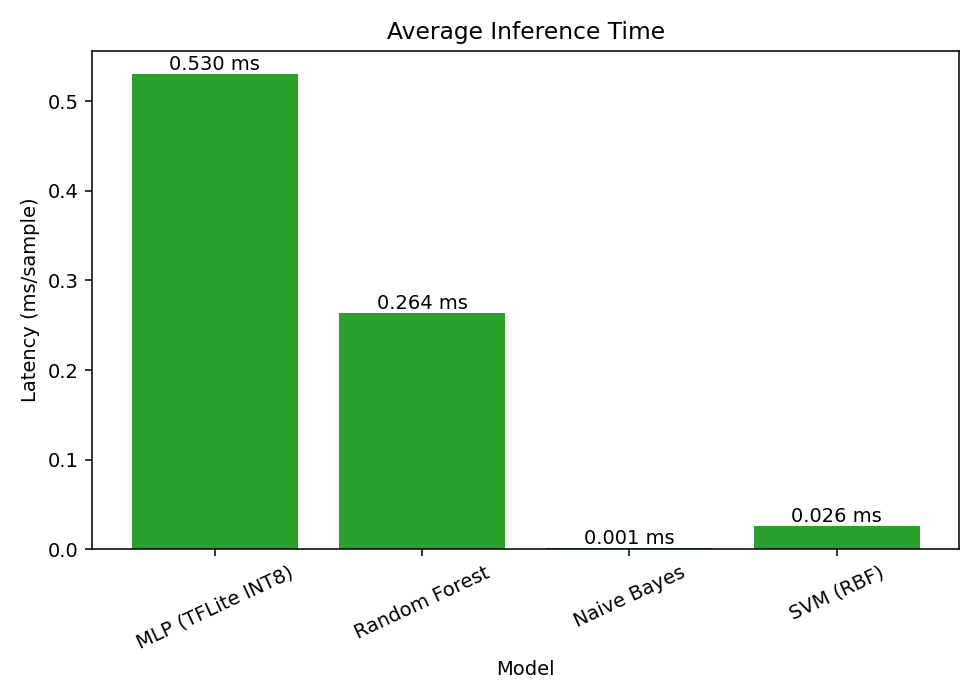
\includegraphics[width=0.8\textwidth]{picture/benchmark_latency.png} 
    \caption{Biểu đồ so sánh thời gian suy luận của các mô hình ML. }
    \label{fig:mips_datapath}
\end{figure}

\begin{figure}[htbp]
    \centering
    % Cài đặt chiều rộng ảnh bằng 80% chiều rộng văn bản
    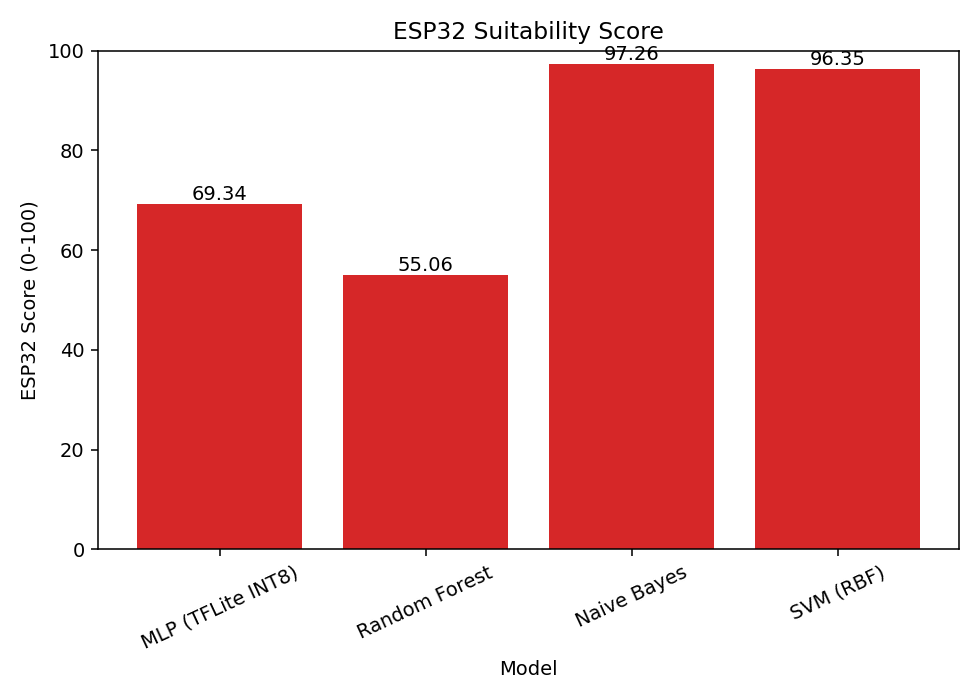
\includegraphics[width=0.8\textwidth]{picture/benchmark_esp32_score.png} 
    \caption{Biểu đồ so sánh điểm số ESP32 của các mô hình ML. }
    \label{fig:mips_datapath}
\end{figure}
\newpage
\subsubsection{Huấn luyện và Xuất mã C (Model Training and C Header Export)}

Dựa trên kết quả đánh giá ở giai đoạn trước, thuật toán Gaussian Naive Bayes (GaussianNB) được lựa chọn nhờ sự cân bằng tối ưu giữa độ chính xác và yêu cầu tài nguyên siêu nhỏ. Thay vì sử dụng các framework biên dịch nặng nề như TensorFlow Lite (TFLite) cho vi điều khiển, hệ thống thực thi một phương pháp triển khai trực tiếp thông qua \texttt{export\_naive\_bayes.py}.

\begin{itemize}
    \item \textbf{Cách triển khai:} GaussianNB không phải là một mạng nơ-ron tiêu chuẩn, do đó việc xuất sang định dạng TFLite không phải là giải pháp phù hợp. Thay vào đó, mô hình được "đóng băng" bằng cách trích xuất các tham số toán học đã học thành các mảng hằng số ngôn ngữ C (C arrays) và tự hiện thực hàm suy luận (score function) trực tiếp trên firmware của ESP32.
    \item \textbf{Chuẩn hóa Z-score:} Trước khi huấn luyện, dữ liệu đầu vào được chuẩn hóa sử dụng phương pháp Z-score. Các tham số trung bình (\texttt{mean}) và độ lệch chuẩn (\texttt{std}) được lưu lại để hệ thống nhúng có thể tiền xử lý dữ liệu cảm biến thực tế theo đúng tỷ lệ toán học.
    \item \textbf{Trích xuất ma trận cốt lõi:} Mô hình được huấn luyện bằng thư viện \texttt{scikit-learn}, sau đó trích xuất các thông số phân phối chuẩn bao gồm:
    \begin{itemize}
        \item Xác suất tiên nghiệm của từng lớp (\texttt{class\_prior\_}).
        \item Kỳ vọng (\texttt{theta\_}) và Phương sai (\texttt{var\_}) của từng đặc trưng (Nhiệt độ, Độ ẩm) tương ứng với từng trạng thái hệ thống.
    \end{itemize}
\end{itemize}



\subsubsection{Kiểm thử mô hình cục bộ (Local Model Testing)}

Bước cuối cùng trước khi triển khai firmware lên phần cứng thực tế là kiểm chứng lại logic suy luận. Việc gỡ lỗi (debug) số học trực tiếp trên vi điều khiển thường tốn thời gian và khó khăn, do đó, \texttt{test\_naive\_bayes.py} được thiết kế để giả lập lại chính xác môi trường tính toán của ESP32 ngay trên máy tính cá nhân.

\begin{itemize}
    \item \textbf{Đồng bộ tham số (Parameter Synchronization):} Hệ thống không tải lại mô hình từ thư viện \texttt{scikit-learn}. Thay vào đó, nó đọc trực tiếp tệp \texttt{naive\_bayes\_model\_metrics.json} (được sinh ra ở phần trước) chứa các ma trận như \texttt{zscore\_mean}, \texttt{zscore\_std}, \texttt{theta}, và \texttt{variance}. Điều này đảm bảo Python và C++ sử dụng chung một "bộ não" tham số.
    \item \textbf{Tái tạo logic toán học:} Hệ thống thực hiện lại các bước tính toán giống hệt mã C sẽ chạy trên ESP32: chuẩn hóa Z-score đầu vào và tính Log-Likelihood dựa trên phân phối chuẩn Gaussian.
    \item \textbf{Đánh giá độ tin cậy (Confidence Scoring):} Trong khi vi điều khiển có thể chỉ cần hàm \texttt{argmax()} để tìm nhãn có điểm cao nhất nhằm tiết kiệm chu kỳ CPU, PC bổ sung thêm hàm \texttt{softmax} để chuyển đổi các giá trị log-likelihood thô thành xác suất phần trăm (\%). Điều này giúp lập trình viên đánh giá độ "tự tin" của mô hình đối với từng dự đoán.
    \item \textbf{Giao diện tương tác (Interactive CLI):} Chương trình cung cấp giao diện dòng lệnh cho phép người dùng nhập tay các giá trị Nhiệt độ và Độ ẩm bất kỳ, sau đó in ra dự đoán tốt nhất (Top 1) kèm theo danh sách xếp hạng các khả năng khác (Top K).
\end{itemize}
\subsubsection{Tối ưu hóa toán học cho vi điều khiển (Log-Likelihood và Log-Sum-Exp)}

Việc triển khai trực tiếp phương trình Gaussian Naive Bayes nguyên bản lên vi điều khiển ESP32 vấp phải hai rào cản kỹ thuật nghiêm trọng:
\begin{enumerate}
    \item \textbf{Tràn số dưới (Underflow):} Xác suất luôn nằm trong khoảng $[0, 1]$. Việc nhân liên tiếp nhiều giá trị xác suất siêu nhỏ sẽ khiến biến \texttt{float} trên ESP32 bị tràn giới hạn lưu trữ và trả về $0.0$, làm hỏng toàn bộ logic phân loại.
    \item \textbf{Chi phí tính toán:} Hàm căn bậc hai (\texttt{sqrt}) và hàm mũ (\texttt{exp}) tiêu tốn rất nhiều chu kỳ xung nhịp (clock cycles), không phù hợp để tính toán lặp lại nhiều lần trên thiết bị biên.
\end{enumerate}

Để giải quyết triệt để, hệ thống áp dụng phép logarit tự nhiên ($\ln$) lên toàn bộ phương trình quyết định. Nhờ đặc tính $\ln(A \times B) = \ln(A) + \ln(B)$, phép nhân đắt đỏ được chuyển hóa thành phép cộng an toàn. Đặt $S_y$ là điểm số (score) của lớp $y$, ta có:

\begin{equation}
S_y = \ln(P(y)) + \sum_{i=1}^{n} \ln(P(x_i|y))
\end{equation}

Khai triển thành phần logarit của hàm mật độ xác suất phân phối chuẩn (Gaussian PDF) cho từng đặc trưng $i$:

\begin{equation}
\ln(P(x_i|y)) = \ln\left( (2\pi\sigma_{y,i}^2)^{-0.5} \cdot \exp\left(-\frac{(x_i - \mu_{y,i})^2}{2\sigma_{y,i}^2}\right) \right)
\end{equation}

Rút gọn biểu thức, ta thu được phương trình Log-Likelihood cuối cùng:

\begin{equation}
\ln(P(x_i|y)) = -0.5 \ln(2\pi\sigma_{y,i}^2) - 0.5 \frac{(x_i - \mu_{y,i})^2}{\sigma_{y,i}^2}
\label{eq:log_likelihood}
\end{equation}

\textbf{Ánh xạ toán học vào mã nguồn C++:} \\
Phương trình (\ref{eq:log_likelihood}) chính là cơ sở để xây dựng hàm \texttt{runNaiveBayes} trong tệp \texttt{tinyml.cpp}. Các phép toán phức tạp đã được tuyến tính hóa hoàn toàn:
\begin{itemize}
    \item Thành phần tiên nghiệm $\ln(P(y))$ tương ứng với lệnh: \\ \texttt{score = logf(fmaxf(kNbClassPrior[c], kNbEpsilon));}
    \item Thành phần $-0.5 \ln(2\pi\sigma_{y,i}^2)$ tương ứng với lệnh: \\ \texttt{score += -0.5f * logf(2.0f * kPi * var);}
    \item Thành phần khoảng cách $-0.5 \frac{(x_i - \mu_{y,i})^2}{\sigma_{y,i}^2}$ tương ứng với lệnh: \\ \texttt{score += -0.5f * (diff * diff / var);}
\end{itemize}
\textit{(Lưu ý: Biến \texttt{var} đại diện cho $\sigma^2$, \texttt{diff} đại diện cho $(x_i - \mu)$, và hằng số \texttt{kNbEpsilon} được cộng thêm nhằm tránh lỗi chia cho 0 hoặc tính $\ln(0)$).}

Cuối cùng, để chuyển đổi điểm số $S_y$ ngược lại thành xác suất phần trăm (\%) mà vẫn tránh được lỗi Underflow, hệ thống sử dụng kỹ thuật \textbf{Log-Sum-Exp}. Thay vì tính trực tiếp $\exp(S_y)$, mã nguồn tìm giá trị lớn nhất (\texttt{max\_score}) và dịch chuyển trục tọa độ:
\begin{center}
    \texttt{class\_probs[c] = expf(class\_scores[c] - max\_score);}
\end{center}
Phép trừ này đảm bảo điểm số cao nhất luôn là $\exp(0) = 1.0$, giữ cho các phép tính xác suất an toàn tuyệt đối trong giới hạn của vi điều khiển.

\subsubsection{Triển khai Firmware trên Vi điều khiển (On-device Deployment)}

Sau khi mô hình được xuất sang mảng C và kiểm chứng logic thành công, bước cuối cùng là tích hợp "bộ não" này vào hệ điều hành thời gian thực (FreeRTOS) trên ESP32. Tệp mã nguồn \texttt{tinyml.cpp} đảm nhiệm vai trò là cầu nối giữa dữ liệu cảm biến thời gian thực và thuật toán Naive Bayes.

\begin{itemize}
    \item \textbf{Kiến trúc đa tác vụ (Multitasking với FreeRTOS):} Thay vì chạy tuần tự trong vòng lặp \texttt{loop()} chặn (blocking) các tiến trình khác, hệ thống gói gọn quá trình suy luận vào một tác vụ độc lập mang tên \texttt{tiny\_ml\_task}.
    \begin{itemize}
        \item Tác vụ này sử dụng cơ chế \textbf{Semaphore} (\texttt{xBinarySemaphoreTinyMLData}) để đồng bộ hóa. Nó sẽ ở trạng thái "ngủ" (Blocked) và không tiêu tốn chu kỳ CPU cho đến khi tác vụ đọc cảm biến (\texttt{temp\_humi\_monitor}) báo hiệu có dữ liệu mới.
    \end{itemize}
    \item \textbf{Động cơ suy luận (Inference Engine):} Hàm \texttt{runNaiveBayes} hiện thực hóa lại chính xác các phương trình toán học đã đề cập ở Phần 4 và Phần 5 bằng thư viện \texttt{<math.h>} của ngôn ngữ C:
    \begin{enumerate}
        \item \textbf{Chuẩn hóa:} Dữ liệu từ cảm biến thực (\texttt{glob\_temperature}, \texttt{glob\_humidity}) được chuẩn hóa Z-score qua hàm \texttt{normalizeInput} sử dụng hằng số \texttt{kNbFeatureMean} và \texttt{kNbFeatureStd}.
        \item \textbf{Tính toán Log-Likelihood:} Sử dụng vòng lặp để cộng dồn xác suất theo công thức phân phối Gaussian.
        \item \textbf{Hàm Softmax \& Argmax:} Tính toán xác suất (\%) cho từng lớp (\texttt{class\_probs}) và chọn ra nhãn có xác suất cao nhất (\texttt{argmax}) làm kết quả dự đoán.
    \end{enumerate}
\end{itemize}


Toàn bộ quá trình từ thu thập, huấn luyện, xuất thông số cho đến tính toán trên vi điều khiển hoàn toàn minh bạch, không phụ thuộc vào hộp đen (black-box API) nào, tối ưu hóa đến từng byte RAM và chu kỳ xung nhịp của vi xử lý.